\documentclass[akbc,twoside,11pt]{article}
\usepackage{akbc}
\usepackage{array}
% \usepackage{ccg-latex}
\usepackage{graphicx}
\usepackage{tabularx}
\usepackage{amsmath}
\usepackage{multirow}
\usepackage{amsfonts} 
\DeclareMathOperator*{\argmax}{argmax} % thin space, limits underneath in displays

\usepackage[colorinlistoftodos]{todonotes}
\newcommand{\ignore}[1]{}
\newcommand{\ensuretext}[1]{#1}
\newcommand{\clabcomment}[3]{\ensuretext{\textcolor{#3}{[#1 #2]}}}
\newcommand{\cjdmarker}{\ensuretext{\textcolor{green}{\ensuremath{^{\textsc{cj}}_{\textsc{d}}}}}}
\newcommand{\cjd}[1]{\clabcomment{\cjdmarker}{#1}{green}}
\newcommand{\tsendee}[1]{\clabcomment{Tsendee:}{#1}{red}}
\newcommand{\raj}[1]{\clabcomment{Raj}{#1}{magenta}}
% \graphicspath{ {images/} }
\ShortHeadings{A survey on Text Style Transfer}{Siddharth Rayabharam}
\akbcheading
\finalcopy % Uncomment for camera-ready version, but NOT for submission.

\graphicspath{ {./assets/} }
% \newcommand{\ignore}[1]{}
% \setlength{\parskip}{0.1cm plus1mm minus1mm}

\begin{document}
\title{A Survey on Text Style Transfer}

% \author{Aishwarya Kamath$^{1}$ \and Rajarshi Das$^{2}$\\
%     $^{1}$Oracle Labs, $^{2}$University of Massachusetts, Amherst \\
%   {\tt aishwarya.kamath@oracle.com, rajarshi@cs.umass.edu} \\}

\author{\name Siddharth Raybharam \email nqr5356@psu.edu \\
        \addr Pennsylvania State University
       }

% \date{April 2018}
\maketitle
\begin{abstract}
Style is an essential component of a sentence. People have a variety of ways of expressing themselves; nevertheless, they adapt the manner in which they talk and write depending on the social setting, the audience, the interlocutor, or the level of formality of the event. Text style transfer is the process of modifying and/or changing the stylistic manner in which a sentence is written while maintaining the meaning of the sentence that was originally written. This process is defined as the task of "text style transfer." Natural language generation uses text style transfer to regulate traits like politeness, emotion, humor, and others. Deep neural models have revived its popularity in natural language processing.

In this paper, we give a comprehensive analysis and assessment of the text style transfer approaches that use deep learning. We highlight the technological developments in deep neural networks that have been the primary impetus behind recent achievements in the fields of natural language comprehension and generation. This paper is structured around two phases in the text style, namely, style classification and style transfer. The discussion focuses on the similarities and differences among the proposed solutions, as well as the challenges and opportunities that are anticipated to guide and stimulate future research in the field.

\noindent\textbf{Keywords: }Text Style Transfer, Deep Learning, Natural Language Processing, Natural Language Generation, Neural Networks
    
\end{abstract}

\section{Introduction}
Culture, individual characteristics, and social context have been attributed to linguistic variations in spoken and written language~\cite{eckert2001style, coupland2007style}. \ignore{In variationist sociolinguistics, the underlying factors contributing to linguistic variations in spoken language have been extensively examined. }An individual's gender, age, education level, personality, and emotional state are some of the personal characteristics that are represented in their writing style. Different people have different ways of expressing themselves, and these characteristics are mirrored in their writing style~\cite{labov1972sociolinguistic}. However, style evolves over time~\cite{eckert2001style} and we adapt to a given social context, audience, communicator, and/or occasion formality~\cite{kiesling1998language}. While direct mapping of sociolinguistic categories is not always possible, natural language understanding and generation research has classified stylistic properties along multiple dimensions.

Text style transfer refers to the process of changing the style of a sentence by rewriting the original sentence in a new style while retaining its semantic content. The range of language types is mirrored in the field's research interests. Some scholars defined style transfer as the ability to change the emotional content of a written document, while others associated it with formality or politeness. Changing the sentiment polarity of a sentence can alter the meaning of a text or transform the message it conveys, but the ability to change the emotional content in a written text should be viewed more in terms of adjusting the tone of a message to be more appropriate, emphatic, and less severe or offensive to the audience or conversational partner. Other researchers have focused their efforts on developing a far more sound understanding of style as a genre, or the language style of a person or a certain social group. 

\ignore{In present and future intelligent interaction systems that comprehend, process, or generate speech or text, language style should be given specific care. When used on discussion forums and comment-based communities, automatic text style adjustment may become even more crucial for users to develop their communication skills (e.g., learning to write formal messages, being more polite), as well as toning down negative sentiment and neutralizing offensiveness.}

Over the course of a decade or two, the work on the subject evolved from a few articles to an active research area. The majority of text style transfer approaches are based on deep neural networks. The research that address the automatic adjustment of a written text's style are crucial to this review. We begin by introducing numerous text styles that have been the subject of text style transfer during the last decade.

\textbf{TODO: A paragraph outlining the paper. Ignore next paragraph}

The paper is organized as follows. After the introductory section, Section~\ref{sec:textual_style} provides a description of various text styles that have been in the focus of the selected research papers. Section~\ref{sec:style_transfer_for_text} gives a formalization of text style transfer and discusses the publicly available datasets suitable for the task at hand. The discussion of a set of measures, which have been proposed as meaningful criteria for evaluating style transfer models, is also presented. Beginning with a brief introduction of several deep neural networks in Section~\ref{sec:deep_neural_networks_for_text_generation}, the discussion of state-of-the-art style transfer methodologies using deep learning is presented in Section~\ref{sec:methods_for_style_transfer}. Section~\ref{sec:challenges} reflects on the challenges style transfer faces and casts light on potential research directions that are expected to further advance the field. Section~\ref{sec:conclusion} concludes the paper.

\section{Text Style and Transfer}
\label{sec:textual_style}

\subsection{Text style}

Individual, societal, and situational factors affect language nuance. Emerging research on automatic style transfer of written text agrees that style is an important aspect of a sentence, signaled by word choice~\cite{argamon2010rest}. We introduce text styles studied in automatic style transfer research. Individual style, and text formality, politeness, offensiveness, and sentiment are briefly described. 

\subsubsection{Personal Style}

Words indicate personality, gender, and age. Several studies imply that language usage differs between demographic groups and that specific terms can be used to identify the author's gender and/or age with 80\% accuracy~\cite{koppel2001automatically}. Female users use more emoticons and terms with positive emotional connotations ~\cite{rao2010classifying}. However, the study shows that younger people use chat-specific e-language and refer to themselves more often, whereas older people use more complex sectences and include more links and hashtags~\cite{nguyen2013old}.

\subsubsection{Formality}

Language style is typically linked to register, or formality, of a text. Formal language is not defined, yet the difference between formal and informal language is clear. Academic writings are more formal than social media. Longer and passive-voiced texts are more formal. Detachment, precision, objectivity, rigidity, and increased cognitive burden characterize formal writing~\cite{sheikha2010automatic} . On the other hand, short words, contractions, and abbreviations are informal~\cite{sheikha2010automatic}. Informal writing is more subjective, less accurate, less informative, and lighter in structure. Automatic formality detection study considers slang, grammatical errors, social distance, and shared knowledge between the writer and the audience. Writing aides can automatically formalize a text.

\subsubsection{Politeness}

The social distance between the writer and the listener influences the politeness of the language. The amount of politeness is vital for keeping a positive face in social interactions with others, and it has a substantial impact on the whole communication experience. Polite and impolite are on opposing ends of the spectrum, yet varying levels of politeness may be employed. Systems for automated politeness adjustment might protect online writing, particularly when someone (unintentionally) produces an unfriendly text that will be received and viewed by others.

\subsubsection{Offensiveness}

The negative repercussions of malevolent online conduct such as hate speech, trolling, and the use of inappropriate language continue to be a recurring issue for practically every social media site. The public, governments, and institutions all want systems and interaction mediators that will automatically recognize, delete, and/or label posts containing objectionable language and hate speech. 

Detecting offensive language is a broad research field that focuses on detecting whether a sentence is offensive or notc~\cite{pavlopoulos2019convai}, or determining the audience (group or person) that is targeted by a message. According to research, the use of particular terms may be associated with inflammatory language. Words like "killed," "fool," and "ignorant" are frequently associated with unpleasant language. Many social media and comment-based news communities applaud the potential advantage of a style transfer mechanism to neutralize harsh statements before they are posted.

\subsubsection{Sentiment}

Emotions affect human behavior, and language frequently reflects them. In many cases, reworking a line with toned-down negative emotions may be preferable. Predictive analytics uses sentiment polarity to determine if a sentence is favorable or negative. Online postings may be used to "sense the mood of a community", public opinion on events, news headline emotions, and political attitude. Sentiment polarity has been used to predict book sales, sales performance, product rankings based on user reviews, stock market predictions based on Twitter moods~\cite{bollen2011twitter}, website popularity, and more.

\subsection{Transfer}

Text style transfer refers to the process of rewriting a sentence in a new style, which involves generating a new (output) sentence with the same explicit meaning as the original (input sentence) but deviating stylistically from the original. Style transfer is used to change, modify, or adapt the way a sentence is written. Table~\ref{tab:tasks} provides instructive examples for each of the style transfer tasks studied in the literature.

\begin{table*}
\centering
\begin{tabularx}{\textwidth} { 
  | >{\raggedright\arraybackslash}X 
  | >{\centering\arraybackslash}X 
  | >{\raggedleft\arraybackslash}X | }
\hline
\textbf{Task} & \textbf{Input Text} & \textbf{Output Text} \\ \hline
\textbf{Sentiment style transfer} & \textit{Great food, but horrible staff and very very rude workers! (negative)} & \textit{Great food, awesome staff, very personable and very efficient atmosphere! (positive)} \\ \hline
\textbf{Politeness transfer} & \textit{Send me the data (non-polite)} & \textit{Could you please send me the data (polite)} \\ \hline
\textbf{Formality transfer} & \textit{Gotta see both sides of the story. (informal)} & \textit{You have to consider both sides of the story. (formal)} \\ \hline
\textbf{Transferring offensive to non-offensive text} & \textit{I hope they pay out the ***, fraudulent or no. (offensive)} & \textit{I hope they pay out the state,	fraudulent or no. (non-offensive)} \\ \hline
\textbf{Personal style transfer} & \textit{My lord, the queen would speak with you, and presently. (shakespearean english)} & \textit{My lord, the queen wants to speak with you right away. (contemporary english)} \\ \hline\end{tabularx}
\caption{\label{tab:tasks} Illustrative examples of selected style transfer tasks.}
\end{table*}

\section{Style Classification}

Due to lack of advances in deep learning neural networks, previous techniques to processing text style were primarily statistical study of language semantics. These statistical methods were used to categorize the documents into different styles. The papers included for this review are concerned with the concept of formality in language and its applications in natural language processing.

Formality is a complex and multidimensional concept that can vary depending on context and audience. Lahiri et al.~\cite{lahiri2011informality} concentrate on one component of formality, namely how closely a sentence adheres to normal grammar and vocabulary rules. They build four datasets, each including 100 documents, from blog postings, news items, academic papers, and internet threads. The authors discovered that the F-score drops across the datasets in the sequence of academic papers, news articles, blog posts, and online threads using the F-score distribution on human annotated sentences and applying the sentence level F-score distribution on each of these datasets. F-score conveys profound formality, which is an essential discovery. The document's \textit{deep formality} grows as additional context is provided. However, adding context necessitates the addition of new words, which makes reading more challenging. Using F-score distribution on an annotated dataset, the authors were able to link F-score with human perception of sentence-level formality, and suggested that some correlation between F-score and readability is expected. 

Sheikha et al.~\cite{sheikha2010automatic} go further describing the contrasts between formal and informal texts. Using 1000 texts from several corpora, the authors were able to extract elements that characterize formal and informal writings, hypothesizing to be a good signal to discern between both styles. The characteristics include a list of formal and informal terms, pronouns, contractions, abbreviations, voice, phrasal verbs, and so on. Using these attributes, the authors tested decision trees, Support Vector Machines (SVM), and the Naive Bayes Algorithm and discovered that these classifiers could predict the classes of new texts with high accuracy of ~98\%.

Ashok et al.~\cite{vikasnovels} use natural language processing techniques to analyze the writing style of a large corpus of novels and then attempt to predict their commercial success based on various stylistic features. The authors use a dataset of over 100,000 novels and their sales rankings to investigate the relationship between writing style and commercial success. They extract various stylistic features such as sentence length, word length, frequency of certain words and phrases, and syntactic complexity. They then use machine learning algorithms such as random forest and support vector machines to predict the commercial success of novels based on these stylistic features. The results of their experiments show that there is indeed a significant relationship between writing style and commercial success. They find that novels with shorter sentences, simpler words, and less syntactic complexity tend to be more commercially successful. Additionally, they find that certain genres such as romance and mystery tend to have more predictive stylistic features than others.

Preotiuc-Pietro et al.,~\cite{preotiuc2016discovering} examine whether there are differences in the way males and females, or younger and older people, write text based on three user attributes: gender, occupational class, and age. They use the Pearson coefficient to determine the level of correlation between the various paraphrases. The authors discovered that the scores are most correlated between users under the age of 25 and users from low occupational classes, as younger users are more likely to have a job with a lower skill level. Intriguingly, the next highest correlation is between low occupational class and female gender. In addition, to predict user attributes, the authors employ the Na\"{i}ve Bayes Classifier and examine ROC AUC and correlation. Age was the feature that showed the highest paraphrase differences in the analysis. Incorporating paraphrase features into gender prediction yields similar outcomes. In the case of occupational class predictions, adding these features actually reduces predictive performance. Age is also the easiest to classify in terms of user trait prediction performance (.901 ROC AUC), followed by occupational class (.870 ROC AUC) and gender (.784 ROC AUC). The authors demonstrated that there are significant changes at the phrase choice level that are both predictive of user traits and intuitive to human annotators.

Lahiri et al., Sheikha et al.,  Ashok et al. and Preotiuc-Pietro et al. demonstrate the diverse applications of formality and style analysis in natural language processing. By analyzing the linguistic features of text, researchers can develop methods for automatically classifying documents, predicting the success of novels, judging the formality of individual sentences and even predicting user attributes. These techniques have the potential to be used in a wide range of fields, from information retrieval and document management to literary analysis and the publishing industry.

\section{RNN}

In next section, we will study the use of machine learning and deep learning techniques in order to transfer or learn the style of the text. The majority of the research articles that are utilized for machine translation make use of some form of Recurrent Neural Networks (RNNs)~\cite{schmidt2019recurrent}. 

RNNs are well suited for machine translation because machine translation involves analyzing words in one language and creating words in another language that convey the original meaning. RNNs can capture long-term dependencies and process sequences of any length, making them ideal for this purpose. In specific the ``Encoder-decoder RNNs" are employed in machine translation. Encoder RNNs convert sentences into fixed-length vectors. The decoder RNN uses this vector, called the "context vector," to create the output sentence word by word. The decoder RNN generates each word in the output sentence using the context vector and relevant input sentence information.

The manner in which information is transported through the network distinguishes Recurrent Neural Networks from Feedforward Neural Networks, commonly known as Multi-Layer Perceptrons (MLPs). While Feedforward Networks send data through the network without using cycles, RNNs use cycles and send data back to themselves. This allows them to enhance the capability of Feedforward Networks to include prior inputs $\mathbf{X}_t$. This difference is visualised on a high level in Figure \ref{fig:rnn}. Note, that here the option of having multiple hidden layers is aggregated to one Hidden Layer block $\mathbf{H}$. This block can obviously be extended to multiple hidden layers.

\begin{figure}
    \centering
    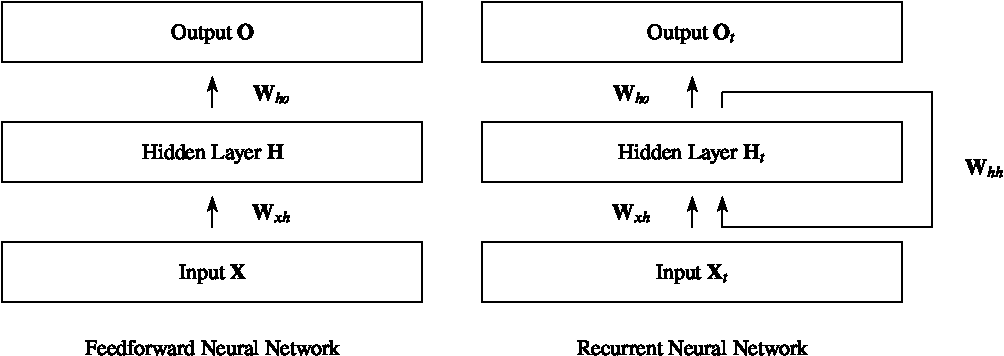
\includegraphics[width=\textwidth]{assets/rnn-cropped.pdf}
    \caption{Visualisation of differences between Feedfoward NNs und Recurrent NNs~\cite{schmidt2019recurrent}}
    \label{fig:rnn}
\end{figure}

We may use the mathematical notation proposed in \cite{zhang2019dive} to explain the process of transmitting information from the previous iteration to the hidden layer. For this, we designate the hidden state and the input at each step $t$ as $\mathbf{H}_{t} \in \mathbb{R}^{n \times h}$ and $\mathbf{X}_t \in \mathbb{R}^{n \times d}$ where $n$ is number of samples, $d$ is the number of inputs of each sample and $h$ is the number of hidden units. Further, we use a weight matrix $\mathbf{W}_{x h} \in \mathbb{R}^{d \times h}$, hidden-state-to-hidden-state matrix $\mathbf{W}_{h h} \in \mathbb{R}^{h \times h}$ and a bias parameter $\mathbf{b}_{h} \in \mathbb{R}^{1 \times h}$. Finally, all of these variables are sent to an activation function $\phi$, which is typically a logistic sigmoid or tanh function, to prepare the gradients for use in backpropagation. When all of these notations are combined, we get Equation \ref{eq:not} as the hidden variable and Equation \ref{eq:outrnn} as the output variable.

\begin{equation}
\label{eq:not}
    \mathbf{H}_{t}=\phi_h\left(\mathbf{X}_{t} \mathbf{W}_{x h}+\mathbf{H}_{t-1} \mathbf{W}_{h h}+\mathbf{b}_{h}\right)
\end{equation}
\begin{equation}
\label{eq:outrnn}
    \mathbf{O}_{t}=\phi_o\left(\mathbf{H}_{t} \mathbf{W}_{h o}+\mathbf{b}_{o}\right)
\end{equation}

\section{Style Transfer}

Cho et al.~\cite{cho2014learning} use RNN to learn phrase representation to capture meaning of entire phrases instead of individual words by encoding a variable length input sequence and then decode the output sequences. The authors also propose a novel hidden unit which is motivated by LSTM unit but is much simpler to compute and implement. This proposed RNN is trained on a large bilingual corpora including Europarl (61M words), news com- mentary (5.5M) and UN (421M) to learn the translation probability of an english phrase to a corresponding french phrase. This model is then used as part of phrase-based statistical machine translation (SMT) framework~\cite{koehn-2005-europarl,marcu-wong-2002-phrase} by scoring each phrase pair in the phrase table. The authors observe that using CSLM~\cite{SCHWENK2007492} and word penality where we penalizes the number of unknown words to neural networks along with RNN has the highest performance in terms of BLEU scores~\cite{papineni2002bleu} among different configurations that were tested to translate phrases from English to French.

Gan et al.~\cite{gan2017stylenet} propose a novel framework named StyleNet to ad- dress the task of generating attractive captions for images and videos with different styles. They devise a novel model component, named factored LSTM, which automatically distills the style factors in the monolingual text corpus. Then at runtime, they explicitly control the style in the caption generation process so as to produce attractive visual captions with the desired style. A factual image/video-caption paired data, and a stylized monolingual text data (e.g., romantic and humorous sentences) are leveraged in order to achieve the goal. StyleNet has a generator and style encoder. Style encoders generate style embeddings from sentences. This embedding conditions the generator. The caption generator takes a noise vector and style embedding as input. A discriminator separates genuine and produced captions after generation. Figure \ref{fig:stylenet} illustrates the learning of Style using the text corpora for different styles. The model is same all different styles except for the styling factor which is trained using mutli-task training on a particular style text corpora.

\begin{figure}[h]
    \centering
    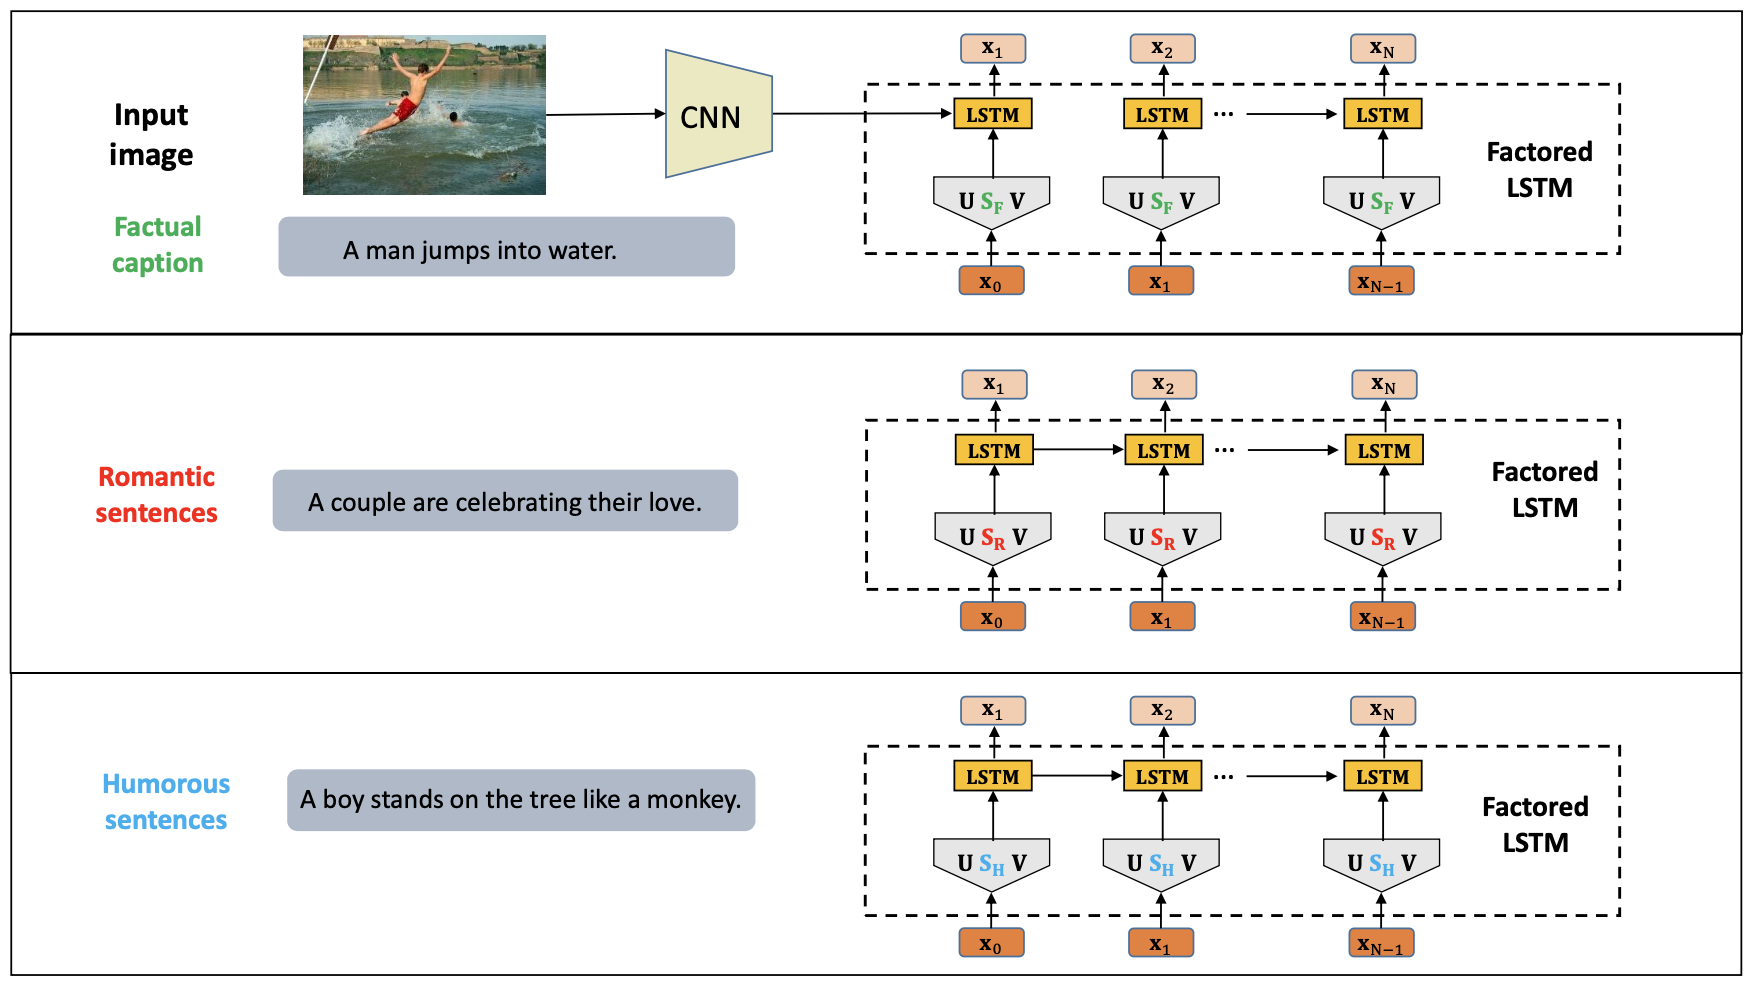
\includegraphics[width=0.8\textwidth]{assets/stylenet}
    \caption{The framework of StyleNet.}
    \label{fig:stylenet}
\end{figure}

StyleNet training uses GAN's adversarial loss and CVAE's reconstruction loss. StyleNet was tested on the COCO dataset, which contains many images with captions. StyleNet captions were compared to vanilla GAN, vanilla CVAE, and a combination of GAN and CVAE without the style encoder. StyleNet outperforms baseline techniques in quantitative and qualitative criteria, the data show.

Prabhumoye et al.~\cite{prabhumoye2018style} propose style transfer of text using back-translation. Back-translation is used to learn two inverse mappings: one from the style of a target sentence to the content of a source sentence, and the other from the content to the original source phrase. By matching the source sentence's content, these inverse mappings increase style transfer. The authors first transfer a sentence to one pivot language and then utilize the pivot language's encoding to train the generative models that correspond to the two styles. They also employ feedback from a pre-trained classifier to direct the generators toward the desired style. This model is called Back-Translated Style Transfer (BST). 

Later in another study~\cite{prabhumoye2018style2} in 2018, Prabhumoye et al. propose an extension to BST to improve the its state-of-the-art performance. They also use feedback mechanism is employed to iteratively refine the style transfer output by allowing users to provide feedback on the generated sentences. The authors analyze the performance of the improved model, MBST+F, along with baseline and BST model on gender transfer, political slant transfer and sentiment modification tasks and observes that the MBST+F performs much better compared to other models.

Cao et al.~\cite{cao2020expertise} reimplement five state-of-the-art models from prior text simplification (TS) and style transfer (ST) studies on both MSD and SimpWiki datasets. The models used are OpenNMT+PT~\cite{klein-etal-2017-opennmt}, UNTS~\cite{sheang-saggion-2021-controllable}, ControlledGen~\cite{hu2018controlled}, DeleteAndRetrieve~\cite{li-etal-2018-delete} and StyleTransformer~\cite{dai-etal-2019-style}. The results demonstrate that the expertise style transfer task is difficult and requires more advanced methodologies than typical style transfer tasks. The basic model outperforms other methods, although it can be improved. The authors then perform a human evaluation research to examine the quality of the generated sentences and discover that the transferred sentences are more layman-like while keeping the content of the expert-written words.


Kashyap et al.~\cite{kashyap2022different} improve the unsupervised attribute transfer by enforcing invariances via explicit constraints. They notice the lack of mechanisms in current methods in text attribute transfer to enforce such constraints between source and the transferred sentence. The authors propose a seq2seq model to encode and decode the text sequences using Adversarially Regularized Auto-encoder (ARAE)~\cite{zhao2018adversarially} which are the auto-encoder variant of Generative Adversarial Networks (GAN). ARAE's have been widely used in text generation and text modeling. The authors test their approach on sentiment, politeness, and formality style transfer tasks. Their model outperforms baseline methods in content preservation and style transfer. The authors further analyze their model's learnt representations, showing that it learns a style-agnostic representation of input sentences independent of the target sentence's style. This analysis illuminates their technique's mechanics and its versatility.

We run the model for 1000 epochs to reduce the training time of the model and compared the results with those of the authors who have run the model for 12000 epochs in the Table~\ref{tab:kashyap}. We can see that the implementation scores are comparatively lower than the authors' run scores. However, the model is really good in detecting the style are transferring them to the texts. Figure~\ref{fig:evalkashyap} indicates the improvement in the accuracy of the model over 1000 epochs.

\begin{table}[h]
\centering
\begin{tabular}{|c|c|c|}
\hline
 & \textbf{Implementation} & \textbf{Authors} \\ \hline
\textbf{Content} & 74.5 & 33.4 \\ \hline
\textbf{Style} & 94.3 & 96.0 \\ \hline
\textbf{Fluency} & 89.1 & 94.4 \\ \hline
\textbf{Joint} & 62.2 & 28.6 \\ \hline
\textbf{GM} & 85.5 & 67.1 \\ \hline
\textbf{BLEU} & 25.7 & 8.7 \\ \hline
\textbf{BERTScore} & 60.1 & 32.4 \\ \hline
\textbf{PPL} & 33.4 & 38.8 \\ \hline
\end{tabular}
\caption{\label{tab:kashyap} Comparison of different scores of styles}
\end{table}

\begin{figure}[h]
    \centering
    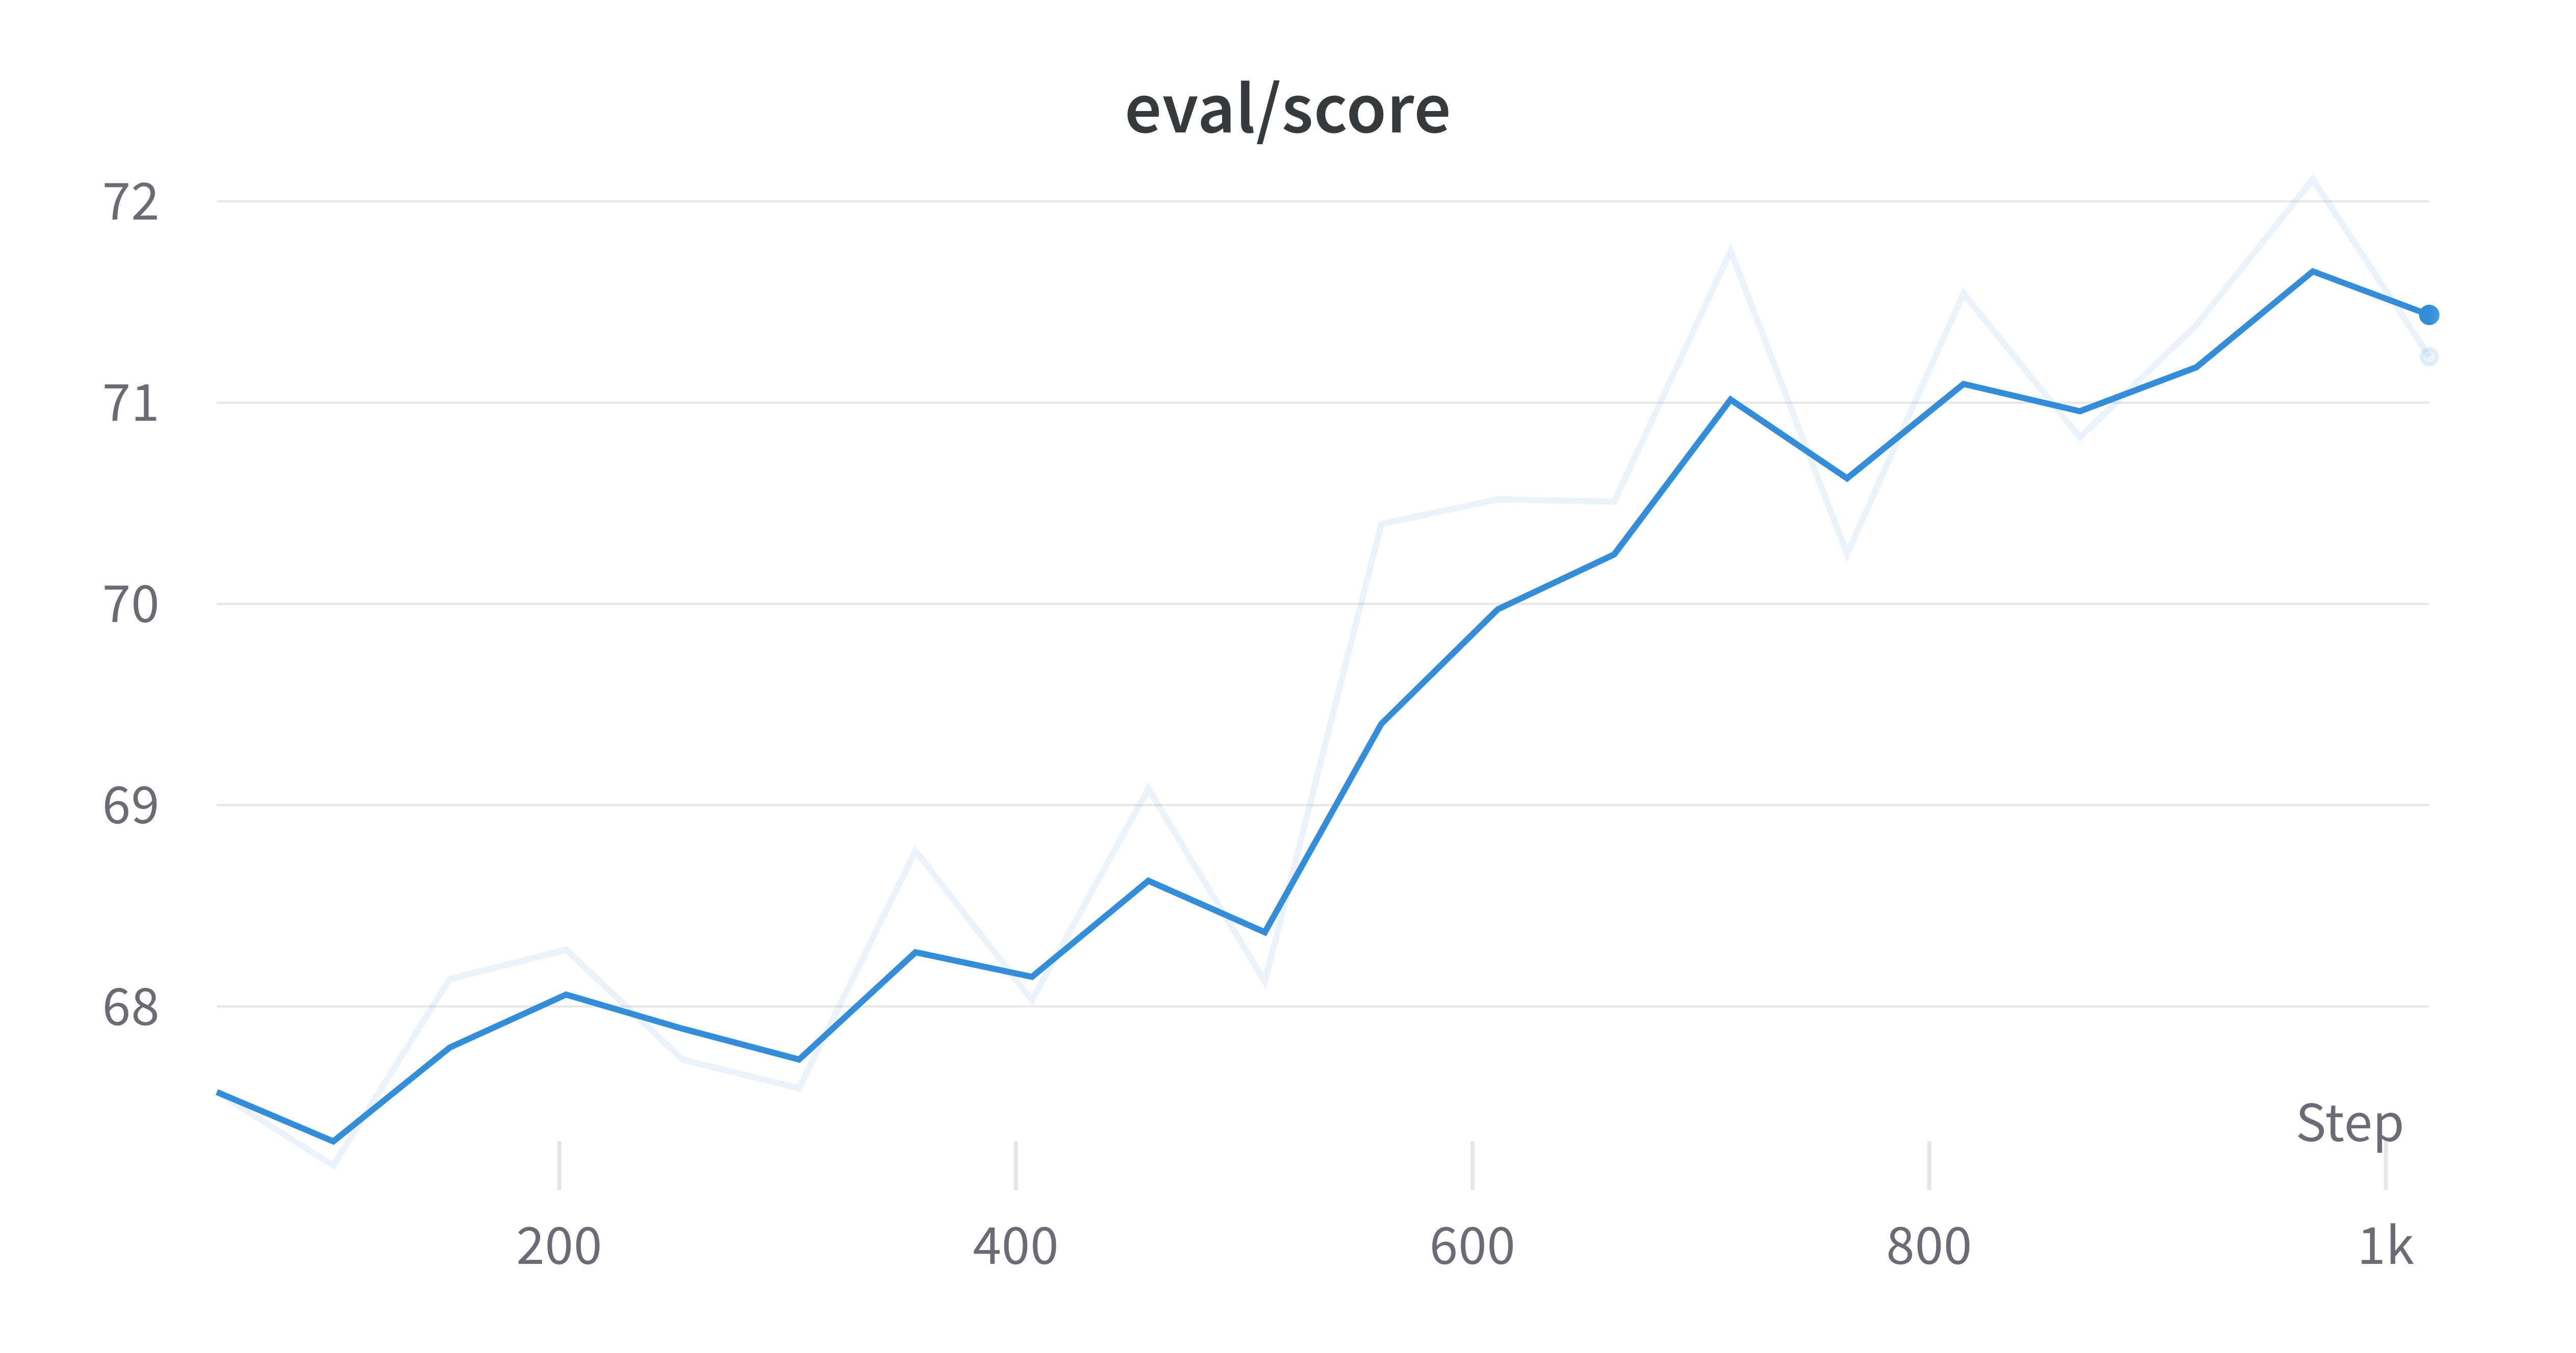
\includegraphics[width=0.8\textwidth]{assets/eval_accuracy_kashyap}
    \caption{The evaluation accuracy of the model over 1000 epochs.}
    \label{fig:evalkashyap}
\end{figure}

Laugier et al.~\cite{laugier2021civil} want to reduce the negative effects of toxic language in online groups by rephrasing toxic communications in a more respectful and civil way. The suggested method is based on a language transformer model that has already been trained and improved using a large dataset of toxic and civil language pairings. The writers use a contrastive learning goal to get the model to come up with rephrases that are both polite and have the same meaning as the offensive original message. The results of the experiments show that the proposed method is more natural and polite than some other ways of rephrasing that are used today. The authors also do an evaluation study on people, which shows that the reworded mean words are seen as more polite and respectful. Overall, the suggested method is a promising way to reduce the negative effects of toxic language in online communities by automatically rephrasing toxic messages in respectful and civil language. This could make the Internet a more welcoming place for everyone. The results showed that the proposed model achieved state-of-the-art performance in terms of fluency and civility while maintaining competitive effectiveness in terms of toxicity reduction. Specifically, the proposed model achieved a 26.6\% reduction in toxicity on the Civil Comments dataset while maintaining a fluency score of 3.56 out of 4, which is the highest among the compared models. Additionally, the authors conducted a human evaluation, which showed that the proposed model generated more civil and polite rephrases compared to the baseline models.

\section{Conclusion}


\ignore{
% Elaborate 
% \section{Terminology}

\section{Task and Salient Components}
\label{sec:task}
\input{sections/task.tex}
\section{Early attempts}
\label{sec:early}
\input{sections/early_attempts.tex}
\section{Semantic parsing from denotations}
\label{sec:qa}
\input{sections/from_denotations.tex}
\section{Alternate forms of supervision}
\label{sec:indirect}
\input{sections/indirect_supervision.tex}
\section{Enter Seq2Seq}
\label{sec:enterseq2seq}
\input{sections/seq2seq.tex}
\section{Learning}
\label{sec:learning}
\input{sections/learning.tex}
\section{Future directions}
\label{sec:conc}
Despite significant progress over the years, there still exist multiple directions worth pursuing. Integrating confidence estimation in the responses from a semantic parser has been largely unexplored and we believe is a useful direction to pursue. In order to have meaningful interactions with conversational agents, knowing when the model is uncertain in its predictions allows for adding human in the loop for query refinement and better user experience. Another promising direction is building semantic parsers that perform well across multiple domains, especially useful when the model needs to be deployed to various user domains that are disparate and lacking sufficient labelled data. Multi-task learning, co-training and fine-tuning across datasets in order to leverage shared representational power as well as being able to generalize to new domains could be a direction to pursue. Leveraging known structure in smarter ways in order to reduce the representational burden on the model and also help it generalize better is currently an area of great interest in the community, with scope for innovation.
% Using static analysis to obtain patterns in the data to augment the the encoder decoder framework to go a step beyond just predicting outputs at a token level could be a promising avenue. 
Since the logical form representation of an utterance is a semantic interpretation of the query, studies for natural language understanding such as RTE could look into leveraging these forms as part of their models or for evaluation. Semantic parsing systems could also be used in lieu of traditional surface form evaluation metrics such as BLEU for machine translation where the evaluation can either be just to check whether the translation is able to produce semantically meaningful sentences or go further and verify whether the result of executing the translated query produces the same denotation. 
}
\bibliography{main}
\bibliographystyle{plainnat}


\end{document}

syntax in semantics- LISA and swabha paper .. elaborate..


%Note about recent attempts to add syntax into models - Emma paper, Swabha paper 